\section{Overview}
\paragraph{}
In Section \ref{mersennekem_intro}, we introduced MersennePKC but did not provide an algorithm for Bob to obtain the plaintext $(A, B) \in \ham_h^n \times \ham_h^n$ given $D = AF + BG$ obtained from multiplying his private key $G$ with the ciphertext $C = A \frac{F}{G}$ sent by Alice. In this chapter, we deduce an algorithm to obtain $(A, B)$ from $D$ by way of an experiment.

\paragraph{}
We make and experimentally confirm two hypotheses:
\begin{itemize}
    \item First Iteration Hypothesis
    \item Second Iteration Hypothesis
\end{itemize}
\paragraph{}
We then use the two hypotheses to deduce an algorithm for computing $(A, B)$ from $D$.

\section{Experimental Strategy}
\paragraph{}
For the entire experiment, we fix cryptosystem parameters $n = 86243$ (a Mersenne prime) and $h = 128$. These parameters were chosen because we desire to have $h = 128$ bits of security, and $n = 86243$ is the smallest Mersenne exponent for which we obtain viable experimental results (for this value of $h$) in Section \ref{expt_results}.

\subsection{Setup} \label{correctness_strategy_setup}
\paragraph{}
The experiment is to be repeated some $N \in \N$ times.
\paragraph{}
For each repetition $\iota$ of the experiment, simulate Alice generating a random plaintext $(A, B) \in \ham_h^n \times \ham_h^n$ by sampling:
\begin{itemize}
    \item $a_1, \dots, a_h$ from $\mathcal{U}(\Z_n)$ without replacement, where $\mu(A) = \sum_{k=1}^h 2^{a_k}$
    \item $b_1, \dots, b_h$ from $\mathcal{U}(\Z_n)$ without replacement, where $\mu(B) = \sum_{k=1}^h 2^{b_k}$
\end{itemize}

\paragraph{}
We also generate Bob's private key $(F, G) \in \ham_h^n \times \ham_h^n$ in the same way, that is by sampling:
\begin{itemize}
    \item $f_1, \dots, f_h$ from $\mathcal{U}(\Z_n)$ without replacement, where $\mu(F) = \sum_{k=1}^h 2^{a_k}$
    \item $g_1, \dots, g_h$ from $\mathcal{U}(\Z_n)$ without replacement, where $\mu(B) = \sum_{k=1}^h 2^{b_k}$
\end{itemize}

\paragraph{}
Let $\alpha_\iota = \{a_1, \dots, a_h\}$. Let $D = AF + BG$.

\paragraph{}
For any subset $U \in \alpha_\iota$ we then define the following functions $\phi_\iota, \phi_{\iota, U}: \Z_n \rightarrow \Z$ in the following way:
\begin{align*}
    \phi_\iota(i) &= Ham(D) - Ham(D - 2^i F)\\
    \phi_{\iota, U}(i) &= Ham(D - \sum_{k \in U} 2^k F) - Ham(D - \sum_{k \in U} 2^k F - 2^i F)
\end{align*}

\subsection{First Iteration: Measurements and Hypothesis}

\paragraph{}
For each repetition $\iota \in \{1, \dots, N\}$, we compute
\begin{align*}
    \mathcal{I}_\iota &= \{(i, \phi_\iota(i) : i \in \alpha_\iota\}\\
    \mathcal{J}_\iota &= \{(i, \phi_\iota(i) : i \not\in \alpha_\iota\}
\end{align*}

\paragraph{}
We then compute the set of all "wanted" points $\mathcal{I}$ and the corresponding frequency map (number of occurrences of each Hamming weight) $\freq{\mathcal{I}}$:
\begin{align*}
    \mathcal{I} &= \bigcup_{\iota = 1}^N \mathcal{I}_\iota\\
    \freq{\mathcal{I}} &= \{ (m, \Delta) : m = |\{ (i, d) \in \mathcal{I} : d = \Delta \}| \}
\end{align*}

\paragraph{}
Additionally, we compute the set of points which are "unwanted", but result in the largest Hamming weight decreases (among all the unwanted points in the same repetition) when chosen. This set $\mathcal{J}_*$, together with corresponding frequency map $\freq{\mathcal{J}_*}$ is given by:
\begin{align*}
    \mathcal{J}_* &= \bigcup_{\iota = 1}^N \{ (i, d) : d = \max \pi_2(\mathcal{J}_\iota) \}\\
    \freq{\mathcal{J}_*} &= \{ (m, \Delta) : m = |\{ (i, d) \in \mathcal{J}_* : d = \Delta \}| \}
\end{align*}

\paragraph{}
We then plot two histograms: $H_\mathcal{I}$ for $\freq{\mathcal{I}}$ and $H_{\mathcal{J}_*}$ for $\freq{\mathcal{J}_*}$ . We fit the normal distributions $N(\mu_\mathcal{I}, \sigma_\mathcal{I}^2)$ and $N(\mu_{\mathcal{J}_*}, \sigma_{\mathcal{J}_*}^2)$ onto $H_\mathcal{I}$ and $H_{\mathcal{J}_*}$ respectively.

\paragraph{\textbf{First Iteration Hypothesis}} Let $X \sim N(\mu_{\mathcal{J}_*}, \sigma_{\mathcal{J}_*}^2)$. We hypothesise that the respective means and variances take on values such that $Pr[X \geq \mu_\mathcal{I}] \approx 10^{-29}$.

\paragraph{}
For each repetition $\iota$, we choose a set of points $U_\iota$ by skimming off all the indices that yield Hamming weight reductions more than $\mu_\mathcal{I}$:
\begin{align*}
    U_\iota = \{ i \in \Z_n : \phi_\iota(i) > \mu_\mathcal{I} \}
\end{align*}

\paragraph{}
Assuming the first iteration hypothesis, $U_\iota \subseteq \alpha_\iota$ with high probability, for each repetition $\iota$.

\subsection{Second Iteration: Measurements and Hypothesis}
\paragraph{}
We then compute:
\begin{align*}
    \mathcal{I}_\iota' &= \{(i, \phi_{\iota, U}(i) : i \in \alpha_\iota \backslash U_\iota\}\\
    \mathcal{J}_\iota' &= \{(i, \phi_{\iota, U}(i) : i \not\in \alpha_\iota \backslash U_\iota\}
\end{align*}

\paragraph{}
We repeat all the calculations as in the first iteration, replacing $\mathcal{I}_\iota$ and $\mathcal{J}_\iota$ by $\mathcal{I}_\iota'$ and $\mathcal{J}_\iota'$ respectively:
\begin{align*}
    \mathcal{I}' &= \bigcup_{\iota = 1}^N \mathcal{I}_\iota'\\
    \freq{\mathcal{I}'} &= \{ (m, \Delta) : m = |\{ (i, d) \in \mathcal{I}' : d = \Delta \}| \}\\
    \mathcal{J}_*' &= \bigcup_{\iota = 1}^N \{ (i, d) : d = \max \pi_2(\mathcal{J}_\iota') \}\\
    \freq{\mathcal{J}_*'} &= \{ (m, \Delta) : m = |\{ (i, d) \in \mathcal{J}_*' : d = \Delta \}| \}
\end{align*}

\paragraph{}
We then plot two new histograms: $H_{\mathcal{I}'}$ for $\freq{\mathcal{I}'}$ and $H_{\mathcal{J}_*'}$ for $\freq{\mathcal{J}_*'}$ . We fit the normal distributions $N(\mu_{\mathcal{I}'}, \sigma_{\mathcal{I}'}^2)$ and $N(\mu_{\mathcal{J}_*'}, \sigma_{\mathcal{J}_*'}^2)$ onto $H_{\mathcal{I}'}$ and $H_{\mathcal{J}_*'}$ respectively.

\paragraph{\textbf{Second Iteration Hypothesis}} Let $Y \sim N(\mu_{\mathcal{J}_*'}, \sigma_{\mathcal{J}_*'}^2)$. We hypothesise that the respective means and variances take on values such that $Pr[Y \geq \mu_{\mathcal{I}'} - 4 \sigma_{\mathcal{I}'}] \approx 10^{-28}$.

\paragraph{}
For each repetition $\iota$, we choose a set of points $U_\iota'$ by skimming off all the indices that yield Hamming weight reductions more than $\mu_{\mathcal{I}'} - 4 \sigma_{\mathcal{I}'}$:
\begin{align*}
    U_\iota' = \{ i \in \Z_n : \phi_{\iota, U_\iota}(i) > \mu_{\mathcal{I}'} - 4 \sigma_{\mathcal{I}'} \}
\end{align*}

\paragraph{}
Assuming the second iteration hypothesis, $U_\iota' \subseteq \alpha_\iota$ with high probability, for each repetition $\iota$.

\section{Experimental Results}\label{expt_results}

\subsection{First Iteration}
\paragraph{}
We plot the histograms $H_{\mathcal{I}}$ (green portion) and $H_{\mathcal{J}_*}$ (red portion) for the first iteration. The data for $H_{\mathcal{I}}$ has a sample mean of $74.5$ and sample variance of $8.64^2$. The data for $H_{\mathcal{J}_*}$ has a sample mean of $25.9$ and sample variance of $4.17^2$.
\paragraph{}
We fit normal distributions to both histograms by method of moments estimation and obtain:
\begin{align*}
    \mu_\mathcal{I} &= 74.5\\
    \sigma_\mathcal{I} &= 8.64\\
    \mu_{\mathcal{J}_*} &= 25.9\\
    \sigma_{\mathcal{J}_*} &= 4.17
\end{align*}

Letting $X \sim N(\mu_{\mathcal{J}_*}, \sigma_{\mathcal{J}_*}^2)$ we use the Gaussian tail bound to obtain:
\begin{align*}
    Pr[X \geq \mu_\mathcal{I}] &= Pr[X - \mu_{\mathcal{J}_*} \geq \mu_\mathcal{I} - \mu_{\mathcal{J}_*}]\\
    &= Pr[X - \mu_{\mathcal{J}_*} \geq 74.5 - 25.9]\\
    &= Pr[X - \mu_{\mathcal{J}_*} \geq 48.6]\\
    &\leq \exp{(-\frac{48.6^2}{2 \sigma_{\mathcal{J}_*}^2})}\\
    &= \exp{(-\frac{48.6^2}{2 \times 4.17^2})}\\
    &\leq 3.20 \times 10^{-30}
\end{align*}

\paragraph{}
This confirms the first iteration hypothesis.

\paragraph{}
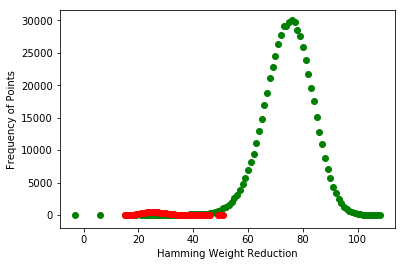
\includegraphics[scale=0.75]{mersennepkc_extraction_first.png}\newline

\subsection{Second Iteration}
\paragraph{}
We plot the histograms $H_{\mathcal{I}'}$ (green portion) and $H_{\mathcal{J}_*'}$ (red portion) for the first iteration. The data for $H_{\mathcal{I}'}$ has a sample mean of $87.5$ and sample variance of $6.65^2$. The data for $H_{\mathcal{J}_*'}$ has a sample mean of $11.9$ and sample variance of $4.35^2$.
\paragraph{}
We fit normal distributions to both histograms by method of moments estimation and obtain:
\begin{align*}
    \mu_{\mathcal{I}'} &= 87.5\\
    \sigma_{\mathcal{I}'} &= 6.65\\
    \mu_{\mathcal{J}_*'} &= 11.9\\
    \sigma_{\mathcal{J}_*'} &= 4.35
\end{align*}

Letting $Y \sim N(\mu_{\mathcal{J}_*'}, \sigma_{\mathcal{J}_*'}^2)$ we use the Gaussian tail bound to obtain:
\begin{align*}
    Pr[Y \geq \mu_{\mathcal{I}'} - 4 \sigma_{\mathcal{I}'}] &= Pr[Y - \mu_{\mathcal{J}_*'} \geq \mu_{\mathcal{I}'} - 4 \sigma_{\mathcal{I}'} - \mu_{\mathcal{J}_*'}]\\
    &= Pr[Y - \mu_{\mathcal{J}_*'} \geq 87.5 - 4 \times 6.65 - 11.9]\\
    &= Pr[Y - \mu_{\mathcal{J}_*'} \geq 49.0]\\
    &\leq \exp{(-\frac{49.0^2}{2 \sigma_{\mathcal{J}_*'}^2})}\\
    &= \exp{(-\frac{49.0^2}{2 \times 4.35^2})}\\
    &\leq 2.80 \times 10^{-28}
\end{align*}

\paragraph{}
This confirms the second iteration hypothesis.

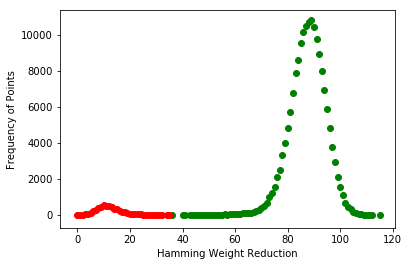
\includegraphics[scale=0.75]{mersennepkc_extraction_second.png}

\section{Deducing the Algorithm}\label{msg_ext_deduction}

At this point, we have experimentally verified the two hypotheses we made earlier. We can now use these hypotheses to obtain an algorithm $\chi_{n, h}$ to extract $(A, B)$ given $D$:
\begin{align*}
\chi_{n, h} &: \mathcal{B}_n \times \ham_h^n \times \ham_h^n \rightarrow \ham_h^n \times \ham_h^n\\
\chi_{n, h} &= (AF + BG, F, G) \mapsto (A, B)
\end{align*}

\subsection{Proposed Algorithm}\label{proposed_algo}
\paragraph{}
Suppose it is known that $A, B, F, G \in \ham_h^n$, where $F$ and $G$ is known to Bob while $A$ and $B$ is not. Suppose Bob has $D = AF + BG \in \mathcal{B}_n$ and wishes to compute $(A, B) \in \ham_h^n \times \ham_h^n$. We propose an procedure EXTRACT-MSG to do so:

\begin{lstlisting}[mathescape=true]
EXTRACT-MSG(n, h, D, F, G):
    A := 0
    B := 0
    
    for k in {0, 1}
        maintain a loop counter $k$
        
        for i: $\Z_n$ in {0, .., n-1}:
            if HAMMING-WEIGHT-DECREASE(D, F, i) >= $\delta_k$:
                set bit i of A
            if HAMMING-WEIGHT-DECREASE(D, G, i) >= $\delta_k$:
                set bit i of B
        
        D := D - (A * F + B * G)
    
    if Ham(A) != h or Ham(B) != h:
        error
    
    return (A, B)
\end{lstlisting}
\newpage

\paragraph{}
The procedure EXTRACT-MSG depends on a threshold $\delta_k$ for $k \in \{0, 1\}$. From the experimental results used to confirm the iteration hypotheses, we set:
\begin{align*}
    \delta_0 &= \mu_{\mathcal{I}}\\
    &= 74.5\\
    \delta_1 &= \mu_{\mathcal{I}'} - 4 \sigma_{\mathcal{I}'}\\
    &= 87.5 - 4 \times 6.65\\
    &= 60.9
\end{align*}

\paragraph{}
The procedure EXTRACT-MSG also depends on a subprocedure:

\begin{lstlisting}
HAMMING-WEIGHT-DECREASE(D, X, i):
    return HAM(D) - HAM(D - X * 2^i)
\end{lstlisting}

\subsection{Probabilistic Correctness of Algorithm}
\paragraph{}
The algorithm has two main iterations, with the main body of each iteration taking place in lines 6-14. We analyse what happens in those two iterations, as well as the error check that takes place in lines 16-17.

\paragraph{}
Let $\alpha$ and $\beta$ be the (unknown) sets, both of size $h$, such that:
\begin{align*}
    A &= \sum_{i \in \alpha} 2^i\\
    B &= \sum_{j \in \beta} 2^j
\end{align*}
To avoid unwieldy prose in the paragraphs that follow, we define the Hamming weight decrease function (the same one as in HAMMING-WEIGHT-DECREASED) by:
\begin{align*}
    \phi &: \mathcal{B}_n \times \ham_h^n \times \Z_n \rightarrow \Z\\
    \phi &= (D, X, i) \mapsto Ham(D) - Ham(D - X * 2^i)
\end{align*}

\paragraph{Probability of Wrong Index Being Chosen}
We first analyse the probability that the algorithm chooses a wrong index to set in either $A$ or $B$. This wrong choice can happen in either of the two iterations of the loop in Line 5.

\paragraph{}
Let $\alpha_0, \beta_0 \subseteq \Z_n$ be the indices chosen and set in the first iteration for $A$ and $B$ respectively. Let $E_{A,0}$ and $E_{B,0}$ be the events that $\alpha_0 \subseteq \alpha$ and $\beta_0 \subseteq \beta$ respectively. By the first iteration hypothesis, we have:
\begin{align*}
    Pr[\overline{E_{A,0}}] &\approx 10^{-29}\\
    Pr[\overline{E_{B,0}}] &\approx 10^{-29}
\end{align*}

\paragraph{}
Let $\alpha_1, \beta_1$ be the indices chosen and set in the second iteration for $A$ and $B$ respectively. Let $E_{A,1}$ and $E_{B,1}$ be the events that $\alpha_1 \subseteq \alpha \backslash \alpha_0$ and $\beta_1 \subseteq \beta \backslash \beta_0$ respectively. By the second iteration hypothesis, we have:
\begin{align*}
    Pr[\overline{E_{A,1}} | \overline{E_{A,0}}] &\approx 10^{-28}\\
    Pr[\overline{E_{B,1}} | \overline{E_{A,0}}] &\approx 10^{-28}
\end{align*}

\paragraph{}
Let $E_A$ and $_B$ be the events that a wrong index is chosen for $A$ and $B$ respectively. We have:
\begin{align*}
    Pr[E_A] &= Pr[E_{A,0}] + Pr[\overline{E_{A,0}}] \times Pr[E_{A,1} | \overline{E_{A,0}}]\\
    &\approx 10^{-29} + (1 - 10^{-29}) \times 10^{-28}\\
    &\approx 10^{-28}\\
    Pr[E_B] &= Pr[E_{B,0}] + Pr[\overline{E_{B,0}}] \times Pr[E_{B,1} | \overline{E_{B,0}}]\\
    &\approx 10^{-28} \text{     (by similar reasoning)}
\end{align*}

\paragraph{}
Let $E$ be the event that the algorithm chooses the wrong index at any time. Then $Pr[E] \leq Pr[E_A] + Pr[E_B] < 2 \times 10^{-28}$. We have therefore established that the algorithm picks the wrong index with extremely low probability. \qed

\paragraph{\textbf{Probability of Insufficient Number of Indices being Chosen}}
Assuming that no incorrect point has been selected, we note that the error condition in line 16 triggers when $\alpha_0 \cup \alpha_1 \not= \alpha$, that is, when there are indices that remain unselected.

\paragraph{}
Let $E'$ be the probability that at least one point that should have been selected but was not. Let $Z \sim N(\mu_{\mathcal{I}'}, \sigma_{\mathcal{I}'}^2)$. Then we have:
\begin{align*}
    Pr[E' | \overline{E}] &= Pr[Z < \mu_{\mathcal{I}'} - 4 \sigma_{\mathcal{I}'}]\\
    &= Pr[\frac{Z - \mu_{\mathcal{I}'}}{\sigma_{\mathcal{I}'}} < -4]\\
    &= \int_{-\infty}^{-4} \frac{1}{\sqrt{2 \pi}} \exp{(-\frac{x^2}{4})} dx\\
    &< 1.34 \times 10^{-4}
\end{align*}

\paragraph{}
We therefore have that the probability of an insufficient number of points is somewhat high (order of $10^{-4}$) compared to the probability of error. This, however, is not a cause for concern since we can simply repeat the loop in line 5 as many times as needed in the rare that an insufficient number of points are selected. \qed

\paragraph{}
We have seen that the message extraction algorithm presented in this section computes the correct $(A,B)$ from $D$ with very high probability (with a small, non-negligible but acceptable chance of needing to run for more than two iterations). We now turn to the runtime of the algorithm.

\subsection{Runtime Of Algorithm}
\paragraph{}
In Subsection \ref{proposed_algo}, we gave an implementation of EXTRACT-MSG and HAMMING-WEIGHT-DECREASE. We first give the time complexity of EXTRACT-MSG in terms of the time complexity of HAMMING-WEIGHT-DECREASE, which we call $T(n)$.

\begin{lemma}
EXTRACT-MSG runs in time $O(n T(n) + nh)$.
\end{lemma}
\paragraph{\textbf{Proof}}
We see that lines 8-14 runs in $O(n T(n))$, since setting bits is $O(1)$ and the loop body (which takes $O(T(n) + 1) = O(T(n))$ is run $n$ times in the loop defined on line 8. Line 14 has multiplications $A*F$ and $B*G$ that take $O(nh)$ since $F$ and $G$ have Hamming weight $h$ and we can simply perform $A*F = \sum_{k = 1}^h A \times 2^{f_k}$ and $B*G = \sum_{k = 1}^h B \times 2^{g_k}$ where $f_1, \dots f_h$ are the bits set in $F$ and $g_1, \dots, g_h$ are the bits set in $G$.

\paragraph{}
The body of the loop in line 5 therefore runs in $O(nT(n) + nh)$, so the entire loop (which makes only a constant number of iterations) runs in $O(nT(n) + nh)$. The check on lines 16-17 run in $O(n)$ since they perform a Hamming weight computation, while the initialisation code on lines 2-3 take $O(n)$ as they allocate memory for bitstrings of length $n$.

\paragraph{}
We can therefore conclude that EXTRACT-MSG runs in $O(nT(n) + nh)$. \qed

\paragraph{}
We note that, from our current implementation, HAMMING-WEIGHT-DECREASE runs in time $O(n)$. This is because all the steps (Hamming weight computation, subtraction, bit shifting) are all linear in the number of bits operated on, which is $n$. This makes the time complexity of EXTRACT-MSG $O(n^2 + nh) = O(n^2)$ since $n > 2 h^2$. With $n = 86243$, the number of operations to be performed is on the order of $10^9$, which is rather large. We therefore propose a functionally-equivalent but more efficient implementation of HAMMING-WEIGHT-DECREASE.

\begin{lstlisting}[mathescape=true]
HAMMING-WEIGHT-DECREASE'(D, X, i):
    compute Y := X * $2^i$
    
    // ensure D > Y, this makes the result off by at most 1
    pad D with an additional bit on the MSB side
    
    //can view D as a bit sequence $d_r \dots d_1$
    //can view Y as an ordered set of indices $\{ y_{j_1}, \dots, y_{j_h} \}$
    
    ham_wt_reduction := 0
    stop := set bit in D with smallest index greater than $y_{j_h}$
    
    for k from h downto 1:
        if $y_{j_k}$ = 0:
            if $d_{j_k}$ = 1:
                stop := $j_k$
            continue
        ham_wt_reduction -= 1
        if $d_{j_k}$ = 1:
            $d_{j_k}$ := 0
        else:
            c := stop - i
            ham_wt_reduction += c
            stop = i
    return ham_wt_reduction
        
\end{lstlisting}

\paragraph{}
The idea behind HAMMING-WEIGHT-DECREASE' is to count the number of places where the Hamming weight could change during subtraction, rather than actually performing the subtraction.
\begin{itemize}
    \item If both the minuend and subtrahend have a bit set at a given index, then the Hamming weight is guaranteed to decrease by exactly one at that index.
    \begin{itemize}
        \item e.g. $110$ - $010$ causes a Hamming weight decrease of one at index $2$
        \item e.g. $11011$ - $1000$ causes a Hamming weight decrease of one at index $4$
    \end{itemize}
    \item If the subtrahend has a bit set at the index but the minuend does not, then the Hamming weight is guaranteed to increase by one less than the number of zeros in the minuend starting from that index and counting upward until the next set bit.
    \begin{itemize}
        \item e.g $10000 - 1$ will cause a Hamming weight increase of $4 - 1 = 3$ since the result becomes $01111$
        \item e.g. $10000 - 10$ will cause a Hamming weight increase of $3 - 1 = 2$ since the result becomes $01110$
    \end{itemize}
\end{itemize}

\paragraph{}
The algorithm searches (the loop in Line 13) all the indices of bits set in the subtrahend (at most $h$ many) and keeps track of the Hamming weight changes when each particular bit of the subtrahend is subtracted from the minuend. When the algorithm terminates, it will return the total Hamming weight change when the entire subtrahend has been subtracted from the minuend, which is what we want.

\begin{claim}
HAMMING-WEIGHT-DECREASE' runs in $O(h)$.
\end{claim}
\begin{proof}
Line 2 runs in $O(h)$ since $X$ has Hamming weight $h$.
Lines 5 and 10 can be done in $O(1)$.
Line 11 can be done in $O(1)$ on average by starting at $d_{j_h}$ and searching upwards, since $D$ is expected to be somewhat dense and no more than a very small number of positions are searched on average.
Every step in Lines 14-24 takes $O(1)$, so the entire loop from Lines 13-24 takes $O(h)$.
\end{proof}

\paragraph{}
Therefore, using HAMMING-WEIGHT-DECREASE' in place of HAMMING-WEIGHT-DECREASE, EXTRACT-MSG has time complexity $O(nh)$. With $n = 86243, h = 128$, this is of order $10^6$, which is very fast on a modern computer.

\paragraph{}
Having obtained an efficient algorithm to compute $(A,B)$ given $D$, we now turn to constructing the key-exchange protocol in the following chapter.